\usepackage[authoryear,round]{natbib}
\usepackage{multirow}

\newcommand{\sheetnum}{%
	05
}
%\setcounter{section}{\sheetnum-3}
\newcommand{\tutorialtitle}{%
    Independent Component Analysis - The Infomax Method
}
\newcommand{\tutorialtitleshort}{%
	Infomax ICA
}
% for slides
\subtitle{\sheetnum \tutorialtitle}

\maxdeadcycles=1000 % Workaround for ! Output loop---100 consecutive dead cycles because of too many figures

% The following use of algroithms is recommended for the notes:
%
%\begin{figure}[!t]
%\removelatexerror
%\begin{algorithm}[H]
    % your algo here
    %\label{alg:algolabel}
    %\caption{algocaption}
%\end{algorithm}
%\end{figure}
%\begin{algorithm}
% Below is the definition for the command \removelatexerror:
\makeatletter
\newcommand{\removelatexerror}{\let\@latex@error\@gobble}
\makeatother

\begin{document} %%%%%%%%%%%%%%%%%%%%%%%%%%%%%%%%%%%%%%%%%%%%%%%%%%%%%%%

\sheet{\sheetnum}{\tutorialtitleshort}

\ttopic{\tutorialtitle}

\begin{frame}
\titlepage
\end{frame}

\begin{frame}
\mode<presentation>{
\tableofcontents[hideallsubsections]
}
\mode<article>{
\tableofcontents
}
\end{frame}

\newpage

% The variable mycolumnleft is set in the minotes class
% The column settings are ignored by the slides
\columnratio{\mycolumnleft,1-\mycolumnleft}
\begin{paracol}{2}
%\setlength{\columnseprule}{0.1pt}
%\setlength{\columnsep}{5em}

\begin{rightcolumn}

\mode<all>

\section{The ICA problem}

\begin{frame}{\secname}

Let $\vec s = (s_1, s_2,...,s_N)^\top$ denote the concatenation of $N$ \underline{independent sources} 
and $\vec x \in \R^N$ describe our observations. $\vec x$ relates to $\vec s$ through a 
\emph{linear transformation} $\vec A$:

\begin{equation}
\label{eq:ica}
\vec x = \vec A \, \vec s
\end{equation}

\notesonly{Again with individual elements and }with $N=2$:
\begin{equation}
 \left( \begin{array}{ll}
			x_1 \\ x_2
		\end{array} \right)
        = \left( \begin{array}{ll}
			a_{11} & a_{12} \\ a_{21} & a_{22}
		\end{array} \right) \cdot \left( \begin{array}{ll}
			s_1 \\ s_2
		\end{array} \right)
	= \left( \begin{array}{l}
		a_{11} s_1 + a_{12} s_2 \\ a_{21} s_1 + a_{22} s_2
	\end{array} \right)
\end{equation}

We refer to $\vec A$ as the \emph{mixing matrix} and \notesonly{\eqref{eq:ica}}\slidesonly{the above} as the \emph{ICA problem}, 
which is recovering $\vec s$ from only observing $\vec x$.

\end{frame}

\begin{frame}{\secname}

The ICA problem can be solved by finding the \emph{unmixing matrix} $\vec W$ such that 
\begin{equation}
\vec s = \vec W \cdot \vec x = \vec A^{-1} \cdot \vec x
\end{equation}

But since we don't have the original mixing matrix $\vec A$ we employ methods of ICA for finding an unmixing matrix $\vec W$ which yields an estimate of the sources, namely $\vec {\hat s}$. 

\begin{equation}
\hat{\vec s} = \vec W \cdot \vec x = \vec A^{-1} \cdot \vec x
\end{equation}

In the case of $N=2$:

\begin{equation}
 \left( \begin{array}{ll}
			\hat s_1 \\ \hat s_2
		\end{array} \right)
        = \left( \begin{array}{ll}
			w_{11} & w_{12} \\ w_{21} & w_{22}
		\end{array} \right) \cdot \left( \begin{array}{ll}
			x_1 \\ x_2
		\end{array} \right)
	= \left( \begin{array}{l}
		w_{11} x_1 + w_{12} x_2 \\ w_{21} x_1 + w_{22} x_2
	\end{array} \right)
\end{equation}

\end{frame}

\begin{frame}{Different methods for solving the ICA problem}

\notesonly{We will discuss several methods for solving the ICA problem:}

\begin{itemize}
\item Methods that maximize the \emph{mutual information} between the observations $\vec x$ and the estimated sources $\vec {\hat s}$ (e.g. Infomax)
\item Methods for maximizing the \emph{non-gaussianity} of $\vec {\hat s}$ (e.g. Kurtosis-based ICA, FastICA)
\end{itemize}

\end{frame}

\begin{frame}{Infomax - Overview}


\clearpage

\underline{Outline for \emph{Infomax} ICA}:
\begin{itemize}
	\item \notesonly{We first look into some }key concepts:
    \begin{itemize}
		\item Uncorrelatedness
		\item \emph{statistical independence}
    \end{itemize}
    \item A primer on information theory
    \begin{itemize}
        \item Entropy
        \item Conditional Entropy
        \item Relative Entropy or \emph{Kullback-Leibler (KL) divergence}
        \item Mutual Information
    \end{itemize}
    \item cost function
    \item ERM
    \item practical aspects
\end{itemize}

\end{frame}

\subsection{Uncorrelatedness}

\begin{frame}{\subsecname}

Correlation measures the linear relationship between two random variables.
\begin{center}
\includegraphics[width=0.7\textwidth]{img/section2_fig3.pdf}
\notesonly{\captionof{figure}{Correlation and uncorrelatedness}}
\end{center}

If no such correlation exists between two random scalar variables $X_1$ and $X_2$. That is, if

\svspace{-3mm}

\begin{align}
\label{eq:uncorr}
\mathrm{Cov}(X_1, X_2) = \E  \lbrack X_1  X_2 \rbrack - \E  \lbrack X_1 \rbrack \, \E \lbrack X_2 \rbrack  &= 0\\
\E  \lbrack X_1  X_2 \rbrack &= \E  \lbrack X_1 \rbrack \, \E \lbrack X_2 \rbrack
\end{align}

$\Rightarrow$ The two variables are \emph{uncorrelated}.

\end{frame}

\subsection{Statistical independence}

\begin{frame}{\subsecname}

Consider the following two random scalar variables $X$ and $Y$:
\begin{center}
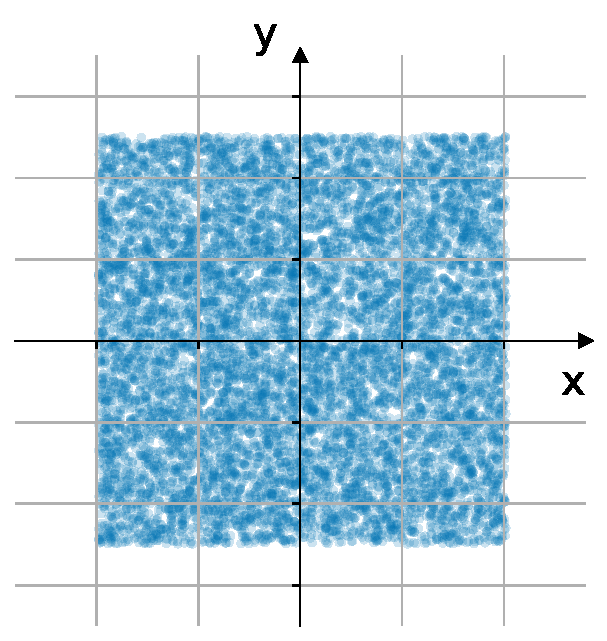
\includegraphics[width=0.4\textwidth]{img/uniform_fixed}
\end{center}

Knowing anything about $X$ reveals absolutely nothing about $Y$, and vice-versa. \notesonly{This is because b}\slidesonly{B}oth variables are \emph{independent}. 

\end{frame}

\begin{frame}{\subsecname}

\only<1>{
Independence requires that the joint probability $p_{X,Y}(x,y)$ factorizes into the product of 
the marginal probabilities $p_X(x)$ and  $p_Y(y)$:

\begin{equation}
\label{eq:statindep}
p_{X,Y}(x,y) = p_X(x) \cdot p_Y(y)
\end{equation}

From this follows:
}
\only<1,2>{

\begin{equation}
\label{eq:statindepexp}
\E  \big\lbrack \, g(x) \cdot h(y) \, \big\rbrack = \E \big\lbrack \, g(x) \, \big\rbrack \cdot \E \big\lbrack \, h(y) \, \big\rbrack  \,,
\end{equation}

where $g(x)$ and $h(y)$ are absolutely integrable functions of $X$ and $Y$.
}
\only<2>{


This can be shown with\notesonly{ the use of \eqref{eq:statindep}}:

\begin{align}
\E  \lbrack \, g(x) h(y) \, \rbrack &= \int_{-\infty}^{\infty} \int_{-\infty}^{\infty} g(x) \, h(y) \, p_{X,Y}(x,y) \, dx \, dy \\
&= \int_{-\infty}^{\infty} \int_{-\infty}^{\infty} g(x) \, h(y)  \, p_X(x) \, p_Y(y) \, dx \, dy \\
&= \int_{-\infty}^{\infty}  g(x) \, p_X(x) dx\, \int_{-\infty}^{\infty} h(y) \, p_Y(y) dy
\,.
\end{align}
}

\end{frame}

\begin{frame}{Uncorrelatedness vs. statistical independence}

\notesonly{
Independence is a much stronger property than decorrelatedness. 
}

\slidesonly{
\begin{center}

\includegraphics[width=0.4\textwidth]{img/meme_stronger}
\end{center}
}

%\pause

If $X$ and $Y$ are independent, they are also uncorrelated, but the same cannot always be said the other way around.



\end{frame}

\begin{frame}{Uncorrelatedness vs. statistical independence: Example}

\only<1>{
Example\footnote{\notesonly{Example obtained} from (Hyv\"arinen, A., \& Oja, E. (2000). Independent component analysis: algorithms and applications. Neural networks, 13(4-5), 411-430.)}:

Assume $X$ and $Y$ are discrete valued and follow a distribution that the pair are with probability 1/4 equal to any of the following
values: (0,1),(0,-1),(1,0),(-1,0). 
}
\begin{center}
	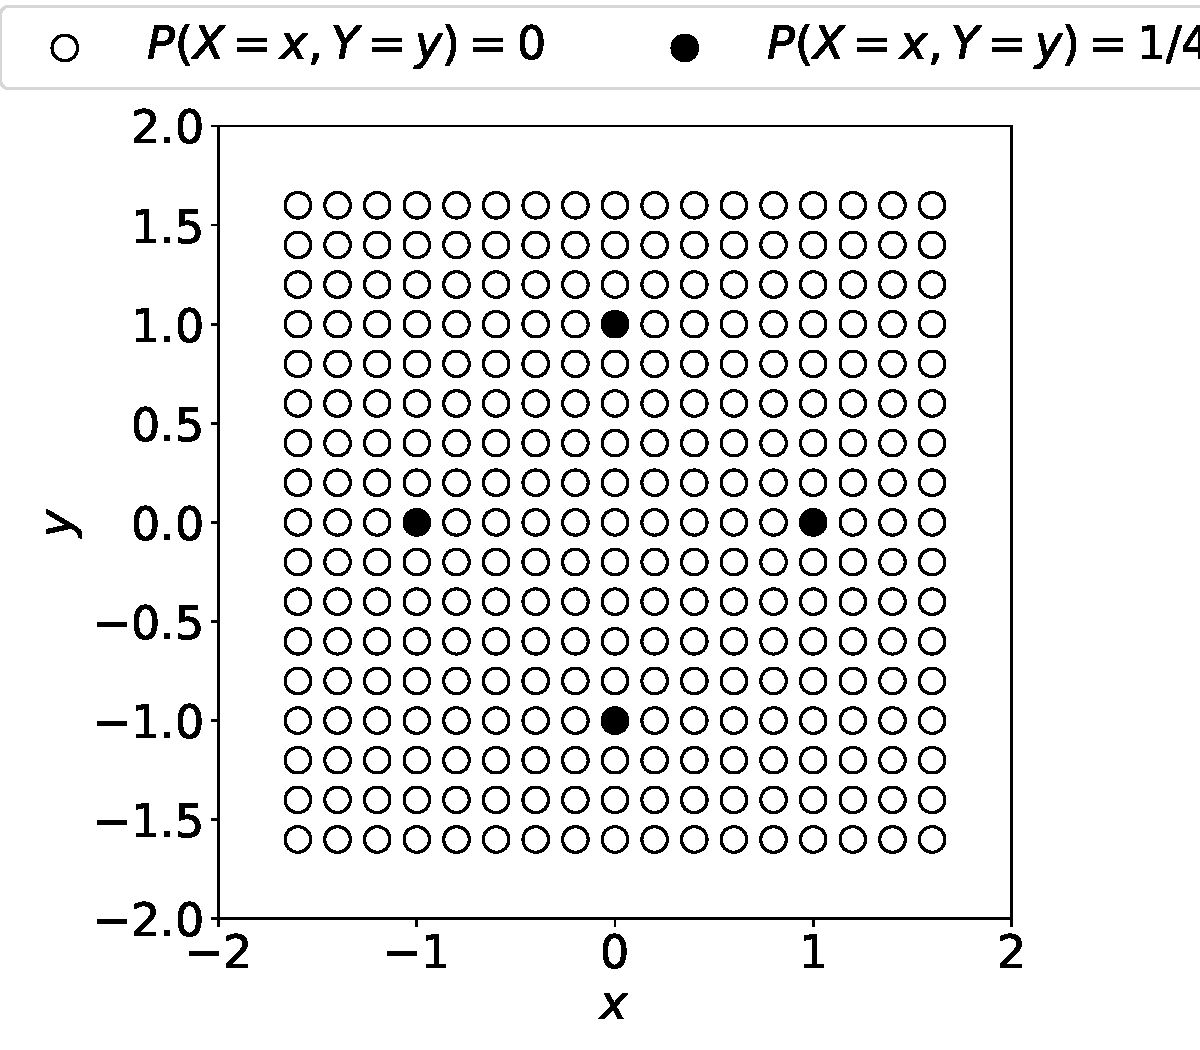
\includegraphics[width=0.4\textwidth]{img/example_decorr_notindep}
	\notesonly{\captionof{figure}{Example for decorrelatedness vs. Independence}}
\end{center}

\only<2-4>{
\question{Are $X$ and $Y$ uncorrelated?}

}
\only<3-4>{

-We check:\\

$\E \lbrack X \rbrack = \frac{1}{4} \cdot (0 + 0 + 1 + (-1)) = 0$\\[2mm]
$\E \lbrack Y \rbrack = \frac{1}{4} \cdot (1 + (-1) + 0 + 0) = 0$\\
}

\notesonly{
- Yes they are uncorrelated.
}

\only<4>{
\slidesonly{
\placeimage{11}{5}{img/meme_yesuncorrelated}{width=3.5cm}
}
}

\end{frame}

\begin{frame}{Uncorrelatedness vs. statistical independence}

\slidesonly{
\begin{center}
	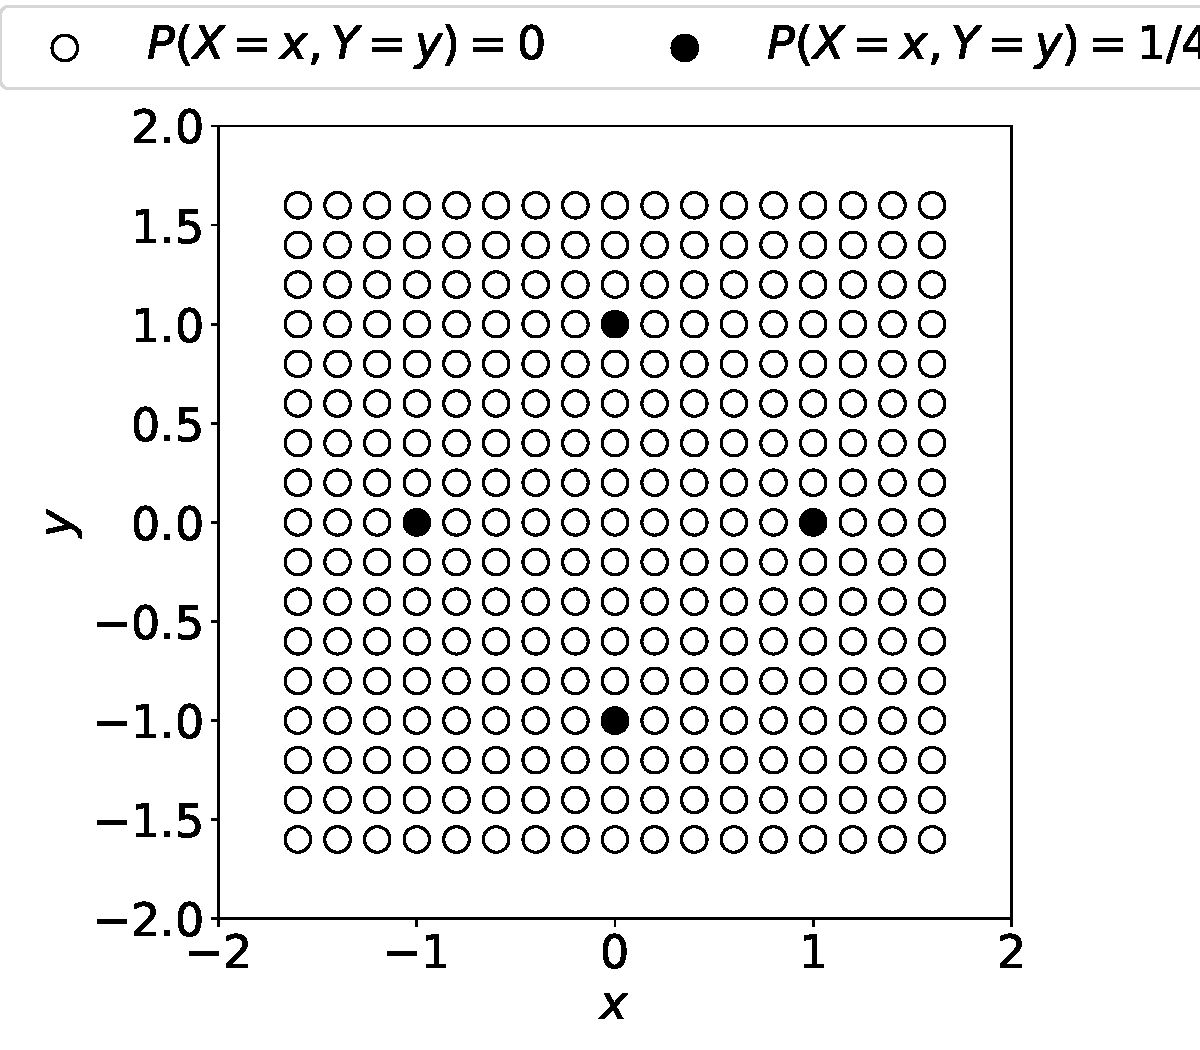
\includegraphics[width=0.4\textwidth]{img/example_decorr_notindep}
	\notesonly{\captionof{figure}{Example for decorrelatedness vs. Independence}}
\end{center}
}

\only<1-3>{
\question{Are $X$ and $Y$ statistically independent?}

}
\only<2-3>{

\notesonly{-As }we calculate $\E  \lbrack \, g(x) h(y) \, \rbrack$ with, e.g., $g(x)=x^2$ and $h(y)=y^2$:\\
$\E \lbrack x^2 \, y^2 \rbrack 
= \frac{1}{4} \cdot \lbrack (0\cdot1) + (0\cdot1) + (1\cdot0) + (1\cdot0) \rbrack = 0 
\ne \frac{1}{4} = \E \lbrack x^2 \rbrack \, \E \lbrack y^2 \rbrack \;,$

\notesonly{we see that }the requirement for independence \notesonly{as in \eqref{eq:statindepexp} }is violated. \notesonly{The variables are uncorrelated but \underline{not} independent.}
}




\only<3>{
\slidesonly{
\placeimage{10.5}{5}{img/meme_butnotindep}{width=4.cm}
}
}

\end{frame}

\clearpage

\begin{frame}

\question{How does statistical independence fit into ICA?}

\pause

- The solution to the ICA problem yields a distribution of the estimated source $\widehat{P}_{\vec s}(\widehat{\vec s})$ that is closest to the factorizing density:

\begin{equation}
\widehat{P}_{s_1, s_2,\ldots,s_N}({\widehat s_1, \widehat s_2,\ldots,\widehat s_N}) = \widehat{P}_{s_1}(\widehat{s_1}) \cdot \widehat{P}_{s_2}(\widehat{s_2}) \cdot \, \ldots \, \cdot \widehat{P}_{s_N}(\widehat{s}_N)
\end{equation}

\pause

\begin{equation}
\label{eq:facts}
\widehat{P}_{\vec s}(\widehat{\vec s}) = \prod_{i=1}^{N} \widehat{P}_{s_i}(\widehat{s_i})  \,.
\end{equation}

To clarify the notation here:\\
\begin{itemize}
%\vspace{-5mm}
%\renewcommand\labelitemi{--}
\setlength\itemsep{0.1em}
\item $\vec s$ describes the independent sources which we do not have.
\item $\widehat{\vec s}$ are the reconstructed sources which we obtain via some unmixing matrix $\vec W$.
\item $\widehat{P}_{\vec s}(\widehat{\vec s})$ is our estimate of the pdf of $\vec s$ which we have approximated using the reconstructions $\widehat{\vec s}$. 
\end{itemize}

\end{frame}

\mode*

\clearpage


\mode<all>
\section{A brief primer on information theory}

\mode<presentation>{
\begin{frame} 
    \begin{center} \huge
        \secname
    \end{center}
    \begin{center}
    Key measures from information theory which play a role in formulating an optimization objective for Infomax ICA
    \end{center}
\end{frame}
}

\notesonly{
Here we go over several measures from information theory which play a role in formulating an optimization objective for Infomax ICA
}

\subsection{Entropy}

\begin{frame}{\subsecname}

Entropy is a measure of uncertainty. It measures the average amount of information conveyed by a message.

\pause

\slidesonly{

\svspace{3mm}

\begin{minipage}{.99\textwidth}
\begin{minipage}{0.3\textwidth}
	\begin{center}
		
\includegraphics[width=0.9\textwidth]{img/meme_entropy1}
	\end{center}
\end{minipage}
\hfill
\begin{minipage}{0.3\textwidth}
	\begin{center}
		
\includegraphics[width=0.7\textwidth]{img/meme_entropy2}
	\end{center}
\end{minipage}
\hfill
\begin{minipage}{0.3\textwidth}
	\begin{center}
		
\includegraphics[width=0.8\textwidth]{img/meme_entropy_none}
	\end{center}
	\end{minipage}
\end{minipage}
}

\end{frame}

\begin{frame}

\begin{block}{Entropy} 
The entropy $H(X)$ of a discrete random variable $X$ is defined by:

\begin{equation}
\label{eq:entropy}
H(X) := - \sum_{x \in \mathcal X} p_X(x)\,\log p_X(x)
\end{equation}

\end{block}

Imagine flipping a biased coin which reveals \textit{tails} most of the time. 
We will no longer be ``surprised'', if we flip the coin again and see it show \textit{tails} \textbf{again}.\\

There is no information gained from flipping the coin another time. There is no uncertainty left.

However, if it were an unbiased coin, we would be equally uncertain of the outcome every time.

\end{frame}

\begin{frame}{Entropy for continuous variables}

We do not have an equivalent measure for continuous random variables. 
However we can resort to the \emph{differential entropy} $h(X)$ of a \textbf{continuous} variable $X$
\footnote{if interested, \citealp[see][Ch~10.2]{haykin1994neural} for the relation between $H(X)$ and $h(X)$.}:

\begin{equation}
\label{eq:entropydiff}
h(X) := - \int_{-\infty}^{\infty} p_X(x)\,\log p_X(x) \, dx 
= - \E \lbrack \log p_X(x) \rbrack
\end{equation}

\end{frame}

%\exercise{Joint Entropy}

%\textbf{Definition:} 
%The joint entropy of $H(X,Y)$ of a pair of discrete random variables $(X,Y)$ with a joint pdf $p_{X,Y}(x,y)$ is defined as:

%\begin{equation}
%\label{eq:entropyjoint}
%H(X,Y) = - \sum_{x \in \mathcal X} \sum_{y \in \mathcal{Y}} p_{X,Y}(x,y)\,\log p_{X,Y}(x,y)
%\end{equation}

\subsection{Conditional Entropy}

\begin{frame}{\subsecname}

Conditional entropy measures entropy of a random variable \textbf{after} one has observed the event of another variable.

\end{frame}

\begin{frame}{\subsecname}

In the case of a system with input $X$ and output $Y$.\\

\svspace{3mm}

\textbf{Definition:} 
The conditional entropy of $H(Y|X)$ of a pair of discrete random variables $(X,Y)$ with a joint pdf $p_{X,Y}(x,y)$ is defined as:

\begin{equation}
\label{eq:entropycond}
H(Y|X) = -\sum_{x \in \mathcal{X}} \sum_{y \in \mathcal{Y}} p_{X,Y}(x,y)\,\log \frac{p_{X,Y}(x,y)}{p_X(x)}
\end{equation}

\question{Where does the definition come from?}

\end{frame}

\begin{frame}{\subsecname: deriving its definition}

\begin{align}
%\label{eq:entropycond}
H(Y|X) 
&= \sum_{x \in \mathcal{X}} p_X(x) H(Y|X=x) \\
&= -\sum_{x \in \mathcal{X}} p_X(x) \sum_{y \in \mathcal{Y}} p(y|x)\,\log p(y|x) \\
&= -\sum_{x \in \mathcal{X}} \sum_{y \in \mathcal{Y}} p_X(x) p(y|x)\,\log p(y|x) \\
&= -\sum_{x \in \mathcal{X}} \sum_{y \in \mathcal{Y}} p_{X,Y}(x,y)\,\log p(y|x) \\
&= -\sum_{x \in \mathcal{X}} \sum_{y \in \mathcal{Y}} p_{X,Y}(x,y)\,\log \frac{p_{X,Y}(x,y)}{p_X(x)} \\
&= -\E_{p_{X,Y}(x,y)} \lbrack \, \log p(Y|X) \, \rbrack
\end{align}

\end{frame}

\begin{frame}{\subsecname}

\question{What does conditional entropy tell us?}

-$H(Y|X)$ represents the amount of uncertainty remaining about a system's output $Y$ \textbf{after} the 
system's input $X$ has been observed.

\pause

\question{What does this mean?} 

\pause

\emph{
$H(Y|X)$ is whatever entropy the output $Y$ has that did not come from the input $X$
}
\only<3>{
\footnote{\cite{bell1995information}}
}.

\question{And what does that mean?}


\end{frame}

\begin{frame}{\subsecname}

\slidesonly{
\emph{
$H(Y|X)$ is whatever entropy the output $Y$ has that did not come from the input $X$
} - \citeauthor{bell1995information}
}

\pause

%\svspace{-5mm}
\begin{center}
\slidesonly{
	\includegraphics<2>[width=0.55\textwidth]{img/aldisain_Plasma_TV}
	\includegraphics<3>[width=0.35\textwidth]{img/Wooden-TV_off}
	\includegraphics<4>[width=0.35\textwidth]{img/Wooden-TV_on}
	\includegraphics<5>[width=0.35\textwidth]{img/Wooden-TV_noise}
}
	\includegraphics<6,8>[width=0.35\textwidth]{img/Wooden-TV_on}
	\includegraphics<7,8>[width=0.35\textwidth]{img/Wooden-TV_noise}
\end{center}

\pause

\svspace{-3mm}

\visible<8>{

\question{Do $X$ and $Y$ have to have an input-output relationship to talk about conditional entropy?}

\notesonly{- No, this is not necessary. An input-output relationship is just a clear and intuitive way to describe dependency between the two variables.}

}

\end{frame}

\begin{frame}{\subsecname}

\slidesonly{
Same as with entropy
\svspace{5mm}
}

For the continuous case, we measure the conditional differential entropy $h(Y|X)$ which is defined as:

\begin{equation}
h(Y|X) = -\int_{-\infty}^{\infty} \int_{-\infty}^{\infty} p_{X,Y}(x,y)\,\log  p_{Y}(y|x) \, dx \, dy
\label{eq:diffentropycondcontinuous}
\end{equation}

\end{frame}

\subsection{Relative Entropy or Kullback-Leibler (KL) divergence}

\begin{frame}{\subsecname}

A measure for how much one probability distribution differs from a reference distribution. 

\textbf{Definition:} 
The relative entropy or Kullback-Leibler divergence between two pdfs $p(x)$ and $q(x)$ is defined as

%\begin{align}
%\label{eq:kldiscrete}
%D_{KL}(p||q) 
%&= \sum{x \in } p_X(x) \log \frac{p_X(x)}{q(x)} \\
%&= -\E_{p_{X}(x)} \,\log \frac{p(X)}{q(X)}
%\end{align}

%for the discrete case. And

\begin{align}
\label{eq:klcont}
\dkl\lbrack\,p\, ||\, q\,\rbrack 
&= \int_{-\infty}^{\infty} p(x) \log \left( \frac{p(x)}{q(x)} \right) dx
\end{align}

for the continuous case.

\end{frame}

\begin{frame}{\subsecname}

\begin{center}
	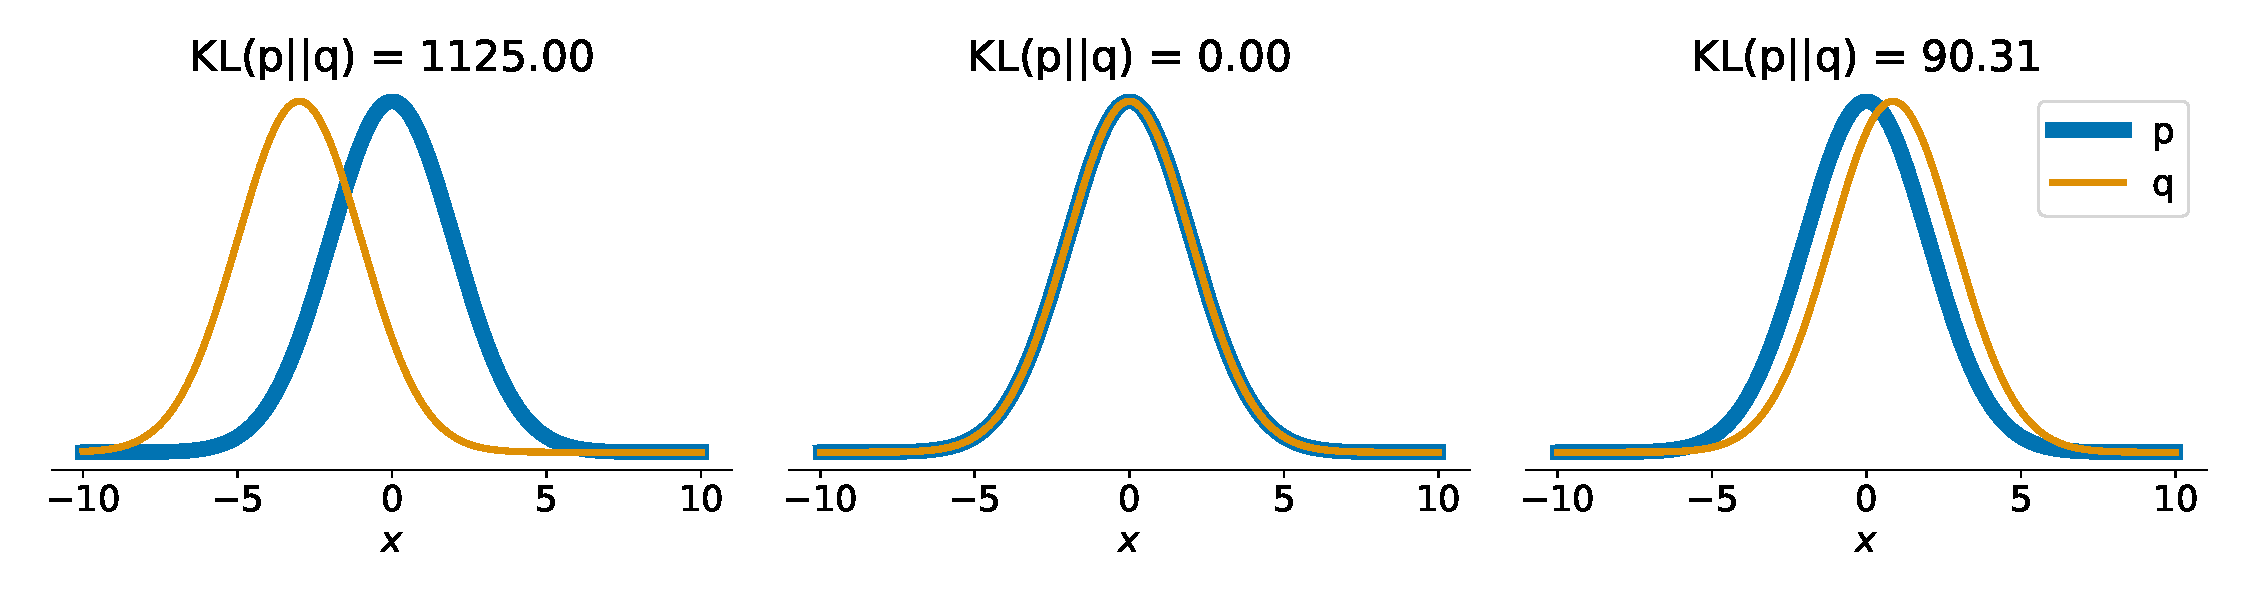
\includegraphics[width=0.8\textwidth]{img/kl_normal}
	
	\pause
	
	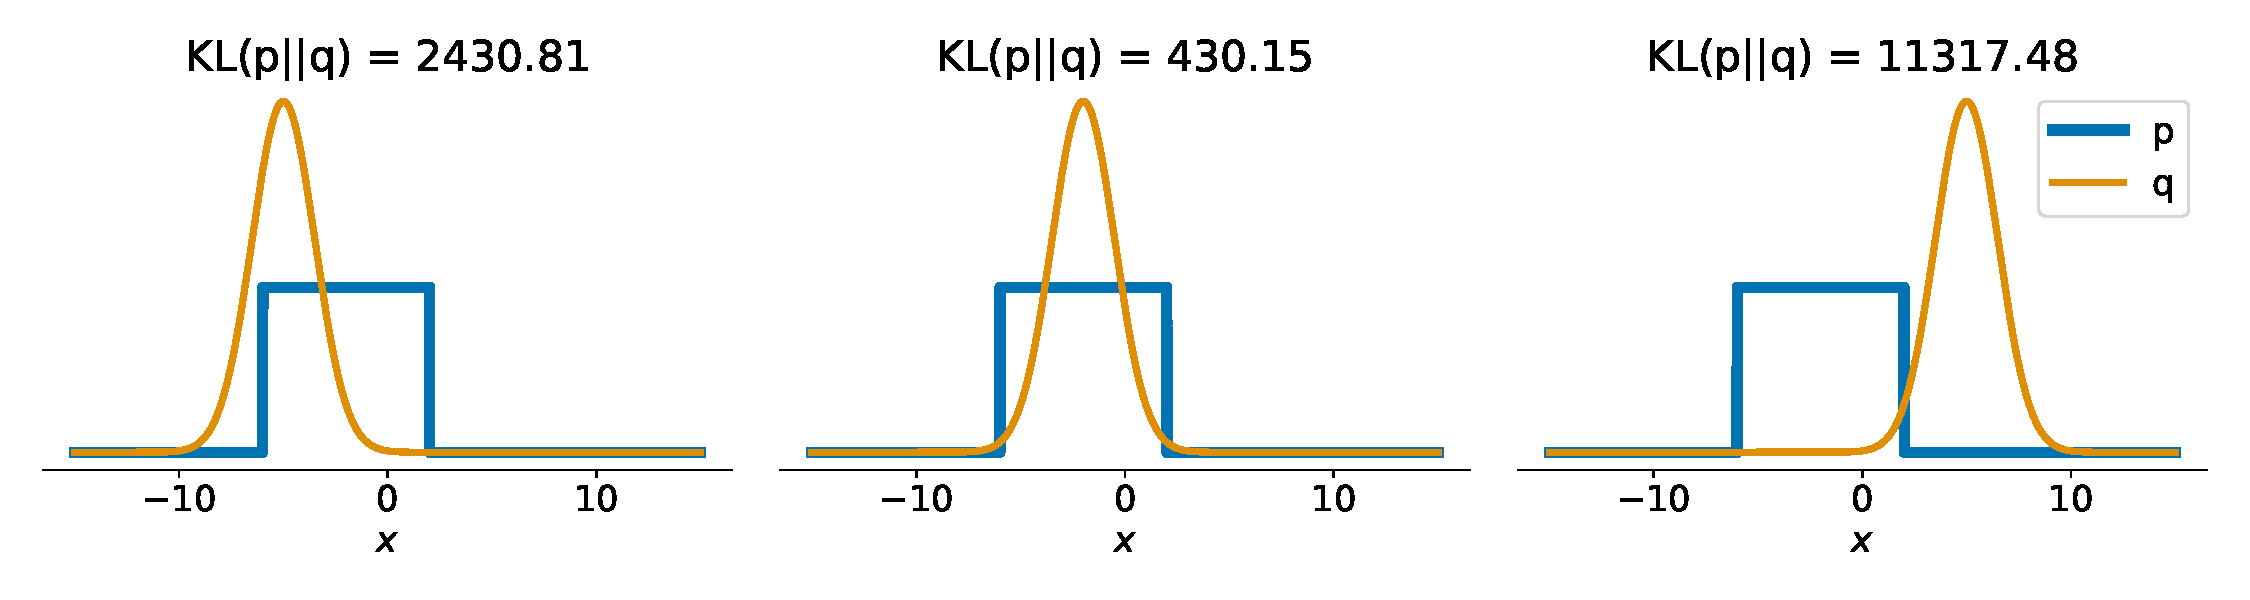
\includegraphics[width=0.8\textwidth]{img/kl_uniform_normal}
	\notesonly{
	\captionof{figure}{Measure the KL divergence between two pdfs.}
	}
\end{center}

\pause 

The KL divergence does not qualify as a distance metric, as it is not symmetric, but it still satisfies other useful metric properties:
\begin{enumerate}
\item non-negative
\item $D_{KL}\lbrack\,p\, ||\, q\,\rbrack = 0$ iff. $p = q$.
\end{enumerate}


\end{frame}


\clearpage 

\begin{frame}{Putting things into the context of ICA}
\notesonly{Let's start putting things into the context of ICA:}

\slidesonly{
\begin{center}
	
\includegraphics[width=0.6\textwidth]{img/meme_puzzle2}
\end{center}
}

\end{frame}

\begin{frame}{Putting things into the context of ICA}
\only<1>{

\slidesonly{
$$
\widehat{\vec {s}} = \vec W \cdot \vec x
$$
}

Recalling the factorization \notesonly{in \eqref{eq:facts} which is based on the assumption that }\slidesonly{\begin{equation}
%\label{eq:facts}
\widehat{P}_{\vec s}(\widehat{\vec s}) = \prod_{i=1}^{N} \widehat{P}_{s_i}(\widehat{s_i})  \,.
\end{equation}}

\notesonly{We want to }\slidesonly{$\Rightarrow$ }formulate an objective for ICA which targets our prior assumption \slidesonly{of independence}\notesonly{that the individual sources are independent from one another.}

\notesonly{The KL-divergence gives us a measure for comparing two distributions. Therefore, we can formulate the objective as }the KL divergence between the joint distribution of the sources and the product of the marginals, specifically:
}
\only<1->{
\begin{equation}
\label{eq:klmin}
	\dkl\lbrack P_{\vec{s}}(\widehat{\vec{s}}),\widehat{P}_{\vec{s}}(\widehat{\vec{s}})\rbrack = 
    \int d \, \widehat{\vec{s}} \; P_{\vec{s}}(\widehat{\vec{s}})
		\ln \frac{P_{\vec{s}}(\widehat{\vec{s}})}{
			\prod_{i = 1}^N \widehat{P}_{s_i}(\widehat{s}_i) }
		\eqexcl \min_{\vec{W}}
\end{equation}
}
\only<2->{

In spite of this being a justified approach for blind source separation, it requires a parametrized density estimate which would make this approach computationally costly.
}
\only<3>{
\slidesonly{
\begin{center}
	
\includegraphics[width=0.35\textwidth]{img/meme_anotherway}
\end{center}
}

} 
\end{frame}

\subsection{Mutual Information}

\begin{frame}{\subsecname}

\begin{itemize}
\item (differential) entropy $h(X)$ represents our uncertainty about $X$ 
and 
\item the conditional (differential) entropy $h(X|Y)$ represents such \textbf{after} observing $Y$.
\end{itemize}

Therefore, the \textbf{difference} between them represents the uncertainty about $X$ \textbf{that is resolved} after observing $Y$,

\pause

which gives us the \emph{mutual information} $I(X,Y)$ between the random variables $X$ and $Y$:

\begin{equation}
I(X,Y) = h(X) - h(X|Y)
\end{equation}

for the continuous case.

\end{frame}

\begin{frame}{\subsecname}

Properties of mutual information:

\begin{align}
\label{eq:mutualcontprops}
I(X,Y) &= h(X) - h(X|Y)\\
&= h(Y) - h(Y|X)\\
%&= h(X) + h(Y) - h(X,Y) \\
&= I(Y,X) \\
&\ge 0
\end{align}

\end{frame}

\subsubsection{Further interpretation for the mutual information}

\begin{frame}{\subsubsecname}

%\begin{align}
%\label{eq:mutualdiscrete}
%I(X,Y) &= H(X) - H(X|Y) \\
%&= \sum{x \in } \sum{y \in } p_{X,Y}(x,y) \, \log \left(\frac{p(x,y)}{p_X(x) p_Y(y)}\right)
%&= H(Y) - H(Y|X) = I(Y,X)
%\end{align}

%for the discrete case. And
\notesonly{Substituting the definitions for $h(X)$ and $h(X|Y)$:}

\begin{align}
\label{eq:mutualcont1}
I(X,Y) 
&= \int_{-\infty}^{\infty} \int_{-\infty}^{\infty} p_{X,Y}(x,y) \, \log \left(\frac{p_X(x|y)}{p_X(x)}\right) dx \, dy \\
\end{align}

\pause

and with the \emph{product rule} $p_{X,Y} = p_X(x|y)\,p_Y(y)$ we get:

\begin{align}
\label{eq:mutualcont2}
I(X,Y)
&= \int_{-\infty}^{\infty} \int_{-\infty}^{\infty} p_{X,Y}(x,y) \, \log \left(\frac{p_{X,Y}(x,y)}{p_X(x) p_Y(y)}\right) dx \, dy
\end{align}

for the continuous case.

\end{frame}




\newpage

\subsection{Relationship between the KL-Divergence and Mutual Information}

\begin{frame}{\subsecname}



This is just to show how to arrive at the same optimization problem\notesonly{ as in \eqref{eq:klmin}} through mutual information.

Recall\notesonly{ the definition of the mutual information between two variables \eqref{eq:mutualcont2}:}

\begin{equation*}
I(X,Y) = \int_{-\infty}^{\infty} \int_{-\infty}^{\infty} {\color{blue}p_{X,Y}(x,y)} \, \log \left(\frac{{\color{blue}p_{X,Y}(x,y)}}{{\color{red}p_X(x) p_Y(y)}}\right) dx \, dy
\end{equation*}

\notesonly{and the definition for the KL divergence from \eqref{eq:klcont}}

\slidesonly{
\begin{align*}
\dkl\lbrack\,p\, ||\, q\,\rbrack 
&= \int_{-\infty}^{\infty} p(x) \log \left( \frac{p(x)}{q(x)} \right) dx.
\end{align*}
}

\pause

We can deduce that:
\begin{equation}
I(X,Y) = D_{KL} \lbrack \, {\color{blue}p_{X,Y}(x,y)} \, || \, {\color{red}p_X(x) p_Y(y)} \, \rbrack
\end{equation}

\end{frame}

\begin{frame}{\subsecname}

\slidesonly{
\begin{equation}
I(X,Y) = D_{KL} \lbrack \, {\color{blue}p_{X,Y}(x,y)} \, || \, {\color{red}p_X(x) p_Y(y)} \, \rbrack
\end{equation}
}

Although $I(X,Y) = I(Y,X)$ the same cannot be said about switching the arguments of the KL-divergence.

\begin{equation}
D_{KL} \lbrack \, {\color{blue}p_{X,Y}(x,y)} \, || \, {\color{red}p_X(x) p_Y(y)} \, \rbrack \ne 
D_{KL} \lbrack \, {\color{red}p_X(x) p_Y(y)} \, || \, {\color{blue}p_{X,Y}(x,y)}\, \rbrack
\end{equation}

The above is only equal if both of them are equal to zero, which is satisfied iff $p_{X,Y}(x,y) = p_X(x) p_Y(y)$.

\notesonly{
This tells us that the mutual information $I(X,Y)$ is equivalent to the KL-divergence between the joint distribution $p_{X,Y}(x,y)$ and 
the product of the pdfs $p_X(x)$ and $p_Y(y)$. A special case of this is what we saw in the first approach, namely the KL-divergence 
between the pdf of a random vector $\widehat {\vec s}$ of length $N$ and the marginal probability density functions for $N$ elements 
$\widehat{s_i}$\footnote{A much smoother walkthrough for this can be found in 
Haykin Ch. 10.5}
}
\slidesonly{
Takeaway:\\
\begin{equation}
\label{eq:klmin}
	\dkl\lbrack{\color{blue}P_{\vec{s}}(\widehat{\vec{s}})},{\color{red}\widehat{P}_{\vec{s}}(\widehat{\vec{s}})}\rbrack = 
    \int d \, \widehat{\vec{s}} \; {\color{blue}P_{\vec{s}}(\widehat{\vec{s}})}
		\ln \frac{{\color{blue}P_{\vec{s}}(\widehat{\vec{s}})}}{
			{\color{red}
			\prod_{i = 1}^N \widehat{P}_{s_i}(\widehat{s}_i) 
			}
			}
		\eqexcl \min_{\vec{W}}
\end{equation}
has an equivalent optimization in terms of mutual information.
}

\end{frame}


\mode*

\clearpage


\mode<all>

\section{The Infomax Principle}

\mode<presentation>{
\begin{frame} 
    \begin{center} \huge
        \secname \\
        (Bell \& Sejnowski, 1995)
    \end{center}
    \begin{center}
    Applying Information theory + density transformation to solve the ICA problem.
    \end{center}
\end{frame}
}

\begin{frame}{The Infomax Principle (Bell \& Sejnowski, 1995)}

\begin{itemize}
\item[\emph{Idea:}] Under certain conditions, maximizing the
  \emph{mutual information} between inputs (mixed signals $\vec x$) and outputs
  (recovered sources $\widehat{\vec s}$) of a system yields \emph{independent} outputs.\\
  
  \svspace{5mm}
  
\item[]
  If sources are independent, then
  transformations of these sources are independent too.\\
  
  \svspace{5mm}
  
\item[]  
  Choosing the transformation such that their marginal distributions become uniform 
  simplifies the computations to find independent sources. i.e. choosing the transformation \\
  
\begin{equation}
\widehat{u}_i = \widehat{f}_i(\widehat{s}_i)
\quad \text{such that} \quad
\widehat{P}_{u_i}(\widehat{u}_i) = \mathrm{const.}
\label{eq:transfconst}
\end{equation}

\end{itemize}

\end{frame}

\subsubsection{Putting Infomax and density transformation together}

\begin{frame}{\subsubsecname}

\notesonly{\underline{Recap on Density Transformation}:\\}

The transformation is found using \emph{conservation of probability}
\begin{equation}
	\widehat{P}_{u_i}(\widehat{u}_i) d \widehat{u}_i 
	\; =  \; \widehat{P}_{s_i} (\widehat{s}_i) d \widehat{s}_i.
\end{equation}
for marginals, and
\begin{equation}
	\widehat{P}_{\vec u}(\widehat{\vec u}) d \widehat{\vec u} 
	\; =  \; \widehat{P}_{\vec s} (\widehat{\vec s}) d \widehat{\vec s}.
\end{equation}
for the joint distribution.


Using the general rule for density transformations and applying it here yields
\begin{equation}
\label{eq:conservation1}
	\widehat{P}_{u_i}(\widehat{u}_i) \quad
	 =  \quad \bigg| 
		\frac{d \widehat{s}_i}{d \widehat{u}_i} \bigg| 
			 \widehat{P}_{s_i}(\widehat{s}_i) \quad
	 =  \quad \frac{1}{\big| \widehat{f}_i^{'} (\widehat{s}_i) \big|} 
		\widehat{P}_{s_i}(\widehat{s}_i)
\end{equation}
where $\left|\frac{d \widehat{s}_i}{d \widehat{u}_i} \right|$ is
called the \emph{functional determinant} of the transformation
$\widehat{f}_i$.

Analogously for the joint distribution:
\begin{equation}
\label{eq:conservation1joint}
	\widehat{P}_{\vec u}(\widehat{\vec u}) \quad
	 =  \quad \bigg| 
		\frac{d \widehat{\vec s}}{d \widehat{\vec u}} \bigg| 
			 \widehat{P}_{\vec s}(\widehat{\vec s})
\end{equation}

\end{frame}

\begin{frame}{Putting Infomax and density transformation together}


\question{What kind of transformation does Infomax need?}

\pause

Infomax requires a transformation resulting in a uniformly distributed
variable with a constant density\notesonly{ (cf. \eqref{eq:transfconst}}.

\slidesonly{
\begin{equation}\widehat{u}_i = \widehat{f}_i(\widehat{s}_i) 
\quad st. \quad
\widehat{P}_{u_i}(\widehat{u}_i) = \mathrm{const.}
\end{equation}
}

\question{What is the density transformation for? }

\pause

-conservation of probability

\end{frame}

\begin{frame}{Putting Infomax and density transformation together}

\svspace{-5mm}

\notesonly{This yields:}

\begin{equation}
  \label{eq:dtufs}
		\widehat{P}_{u_i} (\widehat{u}_i) \; = \;   
		 \frac{1}{\big| \widehat{f}_i^{'} (\widehat{s}_i) \big|} 
		\widehat{P}_{s_i}(\widehat{s}_i) \; \stackrel{!}{=} \; \text{const.} \quad \Rightarrow \quad 
		 \big| \widehat{f}_i^{'} (\widehat{s}_i) \big| =  a \widehat{P}_{s_i}(\widehat{s}_i) 
\end{equation}
and therefore

\svspace{-3mm}

\begin{equation}
\Rightarrow \widehat{f}_i (\widehat{s}_i)
 = \int\limits_{-\infty}^{\widehat{s}_i} dy\; a 
			\widehat{P}_{s_i}(y)
\end{equation}

\begin{figure}[h]
  \centering
  \includegraphics[width=0.7\textwidth]{img/section2_fig15}  
  %\caption{density (pdf) and corresponding distribution function (cdf)}
  \label{fig:cdf}
\end{figure}

\svspace{-2mm}

\question{Why didn't we use the Inverse CDF technique?}

\notesonly{
We don't have an expression for the pdf of the variables to formulate the inverse of its cdf.
}

\end{frame}

\newpage

\begin{frame}{Two Equivalent Approaches to formulating the cost function for Infomax}

\pause

\only<2>{
\slidesonly{
\begin{center}
	
\includegraphics[width=0.4\textwidth]{img/meme_morethanone}
\end{center}
}
}

\slidesonly{
\begin{enumerate}
\item Maximizing mutual information directly - overview only

\pause

\slidesonly{
\begin{center}
	
\includegraphics[width=0.3\textwidth]{img/meme_infomaxisabout}
\end{center}
}

\item Infomax via KL-divergence for the transformed densities
\end{enumerate}


}


\end{frame}

\section{Approach 0: Maximizing mutual information directly - overview only}

\begin{frame}

\notesonly{
One way to formulate the cost function for the Infomax algorithm is to maximize the mutual information directly:
}

\begin{equation}
I(Y,X) = h(Y) - h(Y|X)
\end{equation}

\notesonly{By considering}\slidesonly{Consider} the following relationship between $Y$ and $X$:\\
$Y = g(X;w) + \mathcal{N}$, where $g(\cdot)$ is some invertible transformation parametrized by $w$ and $\mathcal{N}$ is additive noise.

By taking the derivative with respect to the parameter $w$:

\begin{equation}
\frac{\partial}{\partial w} I(Y,X) = \frac{\partial}{\partial w}h(y) - 
\underbrace{\frac{\partial}{\partial w} h(Y|X)}_{= \frac{\partial}{\partial w} h(\mathcal{N}) = 0}
\end{equation}

Maximizing $I(Y,X)$ boils down to maximizing the (differential) entropy of the output $Y$. 

%\notesonly{
%We've seen how mutual information relates to the KL divergence, so we're going to use an approach 
%that operates on the KL-divergence. 
%Whether Infomax by maximizing entropy\footnote{if interested see Bell, A. J., \& Sejnowski, T. J. (1995). An information-maximization approach to blind separation and blind deconvolution. Neural computation, 7(6), 1129-1159.} 
%or finding a factorization via the KL-divergence,
%both are based on the Infomax principle and arrive at the same solution.
%}

\end{frame}

\clearpage

\section{Approach 1: Infomax via KL-divergence for the transformed densities}

\begin{frame}{\secname}

\slidesonly{
\visible<2->{
\vspace{-14mm}
\hspace{8.0cm}
\StickyNote[1.7cm]{
	\begingroup
	\scriptsize
	%\begin{equation}
		%\widehat{P}_{u_i} (\widehat{u}_i) =
		 %\frac{1}{\big| \widehat{f}_i^{'} (\widehat{s}_i) \big|} 
		 %\widehat{P}_{s_i}(\widehat{s}_i)
	%\end{equation}
	\begin{equation}
	{P}_{\vec u}(\widehat{\vec u}) d \widehat{\vec u} 
	\; =  \; {P}_{\vec s} (\widehat{\vec s}) d \widehat{\vec s}
	\end{equation}
\vspace{-2mm}
	\begin{equation}
\label{eq:conservation1joint}
	{P}_{\vec u}(\widehat{\vec u}) \;
	 =  \; \bigg| 
		\frac{d \widehat{\vec s}}{d \widehat{\vec u}} \bigg| 
			 {P}_{\vec s}(\widehat{\vec s})
\end{equation}
\vspace{-2mm}
	\begin{equation}
		\widehat{P}_{u_i}(\widehat{u}_i) := \; \text{const}
	\end{equation}
	\endgroup
}[3.cm] % width
\vspace{-22mm}
}
}

\slidesonly{
\begingroup
\small
}
\begin{align}
  \dkl 
  & = \int d \, \widehat{\vec{s}} P_{\vec{s}}(\widehat{\vec{s}}) \ln \frac{P_{\vec{s}}(\widehat{\vec{s}})}{\prod_i \widehat{P}_{s_i}(\widehat{s}_i)} \slidesonly{\hspace{35mm}}\\
\notesonly{  \intertext{Using the factorization in \eqref{eq:facts}:}}
\visible<2->{
  & = \int d \, \widehat{\vec{s}} P_{\vec{s}}(\widehat{\vec{s}}) \ln \frac{P_{\vec{s}}(\widehat{\vec{s}})}{\widehat{P}_{\vec{s}}(\widehat{\vec{s}})}
\slidesonly{\\}
\notesonly{  \intertext{Applying the density transformation:} }
  %& = &  \int d \, \widehat{\vec{s}} P_{\vec{s}}(\widehat{\vec{s}}) \ln 
  %\frac
  %{P_{\vec{s}}(\widehat{\vec{s}}) \quad \prod_i \frac{1}{f_i' (\widehat{s}_i)}}
  %{\prod_i \widehat{P}_{s_i}(\widehat{s}_i) \quad \frac{1}{f_i' (\widehat{s}_i)}} \\
    %\pause
  & = \int d \, \widehat{\vec{s}} P_{\vec{s}}(\widehat{\vec{s}}) \ln 
  \frac
  {
  \Big|  \frac{d \widehat{\vec u}}{d \widehat{\vec s}} \Big|
  {P}_{\vec u}(\widehat{\vec u}) 
  }
  {
    \Big|  \frac{d \widehat{\vec u}}{d \widehat{\vec s}} \Big|
  \widehat{P}_{\vec u}(\widehat{\vec u}) 
  }
}
\visible<3->{
\slidesonly{\\}
\notesonly{  \intertext{The same factorization in \eqref{eq:facts} equally applies to the transformed variables $\vec u$:} }
  & = \int d \widehat{\vec{u}} P_{\vec{u}} (\widehat{\vec{u}}) 
  \ln 
  \frac
  {P_{\vec{u}} (\widehat{\vec{u}}) }
  {\prod_i  \widehat{P}_{u_i}(\widehat{u_i})} \\
  & = 
  \underbrace{
	  \int d \widehat{\vec{u}} P_{\vec{u}} (\widehat{\vec{u}}) 
	  \ln 
	  {P_{\vec{u}} (\widehat{\vec{u}}) }
  }_{= -H \; \text{(negative entropy)}}\notesonly{\\
  & \quad -}\slidesonly{\;\; - \;\;}
  \underbrace{
	  \int d \widehat{\vec{u}} P_{\vec{u}} (\widehat{\vec{u}}) 
	  \bigg( \ln
	  {\prod_{i=1}^{N}
	  \overbrace{ 
		\widehat{P}_{u_i}(\widehat{u_i}) 
	  }^{\substack{\text{const.\;}\notesonly{ a \\\text{\;see \eqref{eq:dtufs}}}}}} 
	  \bigg)
	  }_{\text{constant}}
}
\end{align}
\slidesonly{
\endgroup
}

\end{frame}



\begin{frame}

This gives us a new but equivalent formulation for the Infomax optimization problem:
\begin{equation}\label{eq:infomax}
  H = -\int d \widehat{\vec{u}} P_{\vec{u}} (\widehat{\vec{u}})
  \ln P_{\vec{u}} (\widehat{\vec{u}}) \eqexcl \max_{\vec W} 
\end{equation}

using the transformed estimated sources
\begin{equation}
\widehat{u}_i := \widehat{f}_i \big( \underbrace{ \vec{e}_i^\top
		\vec{W} \, \vec{x}  }_{= \widehat{s_i} } \big) 
\end{equation}

where $\vec e_i$ is a \emph{basis} vector where the $i$-th element is equal to 1 and all other elements are zero.
Example for $\vec e_i$ for selecting the $i$-th reconstruction with 2D observations:
\begin{equation}
\textcolor{blue}{\hat {\mathrm{s}}_2} =
\overbrace{
\big( \, 0 \;\; \textcolor{blue}{1} \, \big) 
}^{\vec e_2^\top}
	\left( \begin{array}{ll}
	{\mathrm{w}_{11}} & {\mathrm{w}_{12}} \\
		{\mathrm{w}_{21}} & {\mathrm{w}_{22}} 
	\end{array} \right)
	\left( \begin{array}{ll}
		\mathrm{x}_1 \\ \mathrm{x}_2
	\end{array} \right)
	= \big( \, 0 \;\; \textcolor{blue}{1} \, \big)
	\left( \begin{array}{ll}
		\hat {\mathrm{s}}_1 \\ \textcolor{blue}{\hat {\mathrm{s}}_2}
	\end{array} \right)
\end{equation}

\end{frame}

\begin{frame}

\question{What does this tell us?}

\pause

This tells us that 
\begin{itemize}
\item we can produce statistically independent sources $\widehat {\vec s}$ 
by maximizing the entropy of their transformation $\vec u$.
\only<3>{
\item maximizing the entropy of $\vec u$ is equivalent minimizing \notesonly{\eqref{eq:klmin}}
}

\begingroup
\footnotesize
\begin{equation}
\label{eq:klminequivh}
\visible<2->{
 \quad H(\vec u) \eqexcl \max_{\vec W} 
 }
 \visible<3->{
  \;\; \Leftrightarrow \;\;
 	\dkl\lbrack P_{\vec{s}}(\widehat{\vec{s}}),\widehat{P}_{\vec{s}}(\widehat{\vec{s}})\rbrack = 
    \int d \, \widehat{\vec{s}} \; P_{\vec{s}}(\widehat{\vec{s}})
		\ln \frac{P_{\vec{s}}(\widehat{\vec{s}})}{
			\prod_{i = 1}^N \widehat{P}_{s_i}(\widehat{s}_i) }
		\eqexcl \min_{\vec{W}} 
 }
\end{equation}
\endgroup
\pause

\item It is equivalent to maximizing the mutual information.
Recall ``Maximizing $I(Y,X)$ boils down to maximizing the entropy of the output $Y$.''.
We now know that $Y$ is $u_i$ and $X$ is an observed variable $x_i$.

\pause

Now that we've found the cost function for our learning algorithm. 
We build something that can learn to solve the ICA problem.

\end{itemize}

\end{frame}

% -----------------------------------------------------------------------------

\mode*

\clearpage


\mode<all>
\section{Empirical Risk Minimization}

\mode<presentation>{
\begin{frame} 
    \begin{center} \huge
        \secname
    \end{center}
    \begin{center}
    Optimize the cost function using training data.
    \end{center}
\end{frame}
}

\begin{frame}{Our model for solving the ICA problem}

Consider the following perceptron network with $N$ inputs and $N$ outputs:
\begin{figure}[ht]
\centering
\includegraphics[width=4.5cm]{img/section2_fig16}
%\caption{$N-N$ perceptron network}
\end{figure}
where
\svspace{-4mm}
\begin{equation}
\widehat{u}_i := \widehat{f}_i 
	\big( 
		s_i 
	\big) = \underbrace{
	\widehat{f}_i 
	\Big( \sum_{j=1}^{N} \mathrm{w}_{ij} 
		\mathrm{x}_j 
	\Big) }_{
	\substack{
		\text{often a} \\
		\text{sigmoid function}\\
		\text{or\;} \tanh}
	}
\end{equation}
and observations:
\svspace{-4mm}
\begin{equation}
\vec{x}^{(\alpha)} \in \mathbb{R}^N, 
		\quad \alpha = 1, \ldots, p
\end{equation}
The weights $w_{ij}$ will be determined through inductive learning.

\end{frame}

\begin{frame}

Deriving the cost function for this network to find the Infomax solution:
\begin{equation}
\label{eq:conservationvec}
	P_{\vec{u}} (\widehat{\vec{u}}) d \widehat{\vec{u}}
		= P_{\vec{x}}(\vec{x}) d \vec{x}
\end{equation}
\begin{align}
\label{eq:uxj}
	P_{\vec{u}} (\widehat{\vec{u}}) 
	& = \left| \det \frac{d \vec{x}}{d \widehat{\vec{u}}} \right|
		P_{\vec{x}}(\vec{x}) \\
	& = \frac{P_{\vec{x}}(\vec{x})}{ \left| \det
		\frac{d \widehat{\vec{u}}}{d \vec{x}} \right|}\\
    & = \frac{P_{\vec{x}}(\vec{x})}{|\det \vec{J}\,|}
\end{align}
with elements of the Jacobian $\vec J$ given as
\slidesonly{
	\begingroup
	\small
}
\begin{align}
\label{eq:jacobelement}
 J_{ij}=
 \frac{\partial \widehat{u}_i}{\partial \mathrm{x}_j}
	& = \frac{\partial}{\partial \mathrm{x}_j} 
		\widehat{f}_i \bigg( \sum\limits_{k = 1}^N \mathrm{w}_{ik} 
		\mathrm{x}_k \bigg) \notesonly{\\
	&} = \mathrm{w}_{ij} \widehat{f}_i^{'} \bigg( \sum\limits_{k = 1}^N 
		\mathrm{w}_{ik} \mathrm{x}_k \bigg).
\end{align}
\slidesonly{
	\endgroup
}

We therefore obtain for the value of the Jacobian determinant
\slidesonly{
	\begingroup
	\footnotesize
}
\begin{equation} \label{eq:functionalDeterminant}
|\det \vec {J}\,| = 
	\Big| \det \frac{\partial \widehat{\vec{u}}}{\partial \vec{x}} \Big|
	= |\det \vec{W}\, | \prod\limits_{l = 1}^N  \widehat{f}_l^{'} \Bigg( 
		\sum\limits_{k = 1}^N \mathrm{w}_{lk} \mathrm{x}_k \Bigg).
\end{equation}
\slidesonly{
	\endgroup
}

\end{frame}

\clearpage

\begin{frame}

\slidesonly{
\visible<1->{
\vspace{-7mm}
\hspace{8.0cm}
\StickyNote[1.7cm]{
	\begingroup
	\scriptsize
\begin{equation}
%\label{eq:conservationvec}
	P_{\vec{u}} (\widehat{\vec{u}}) d \widehat{\vec{u}}
		= P_{\vec{x}}(\vec{x}) d \vec{x}
\end{equation}
\begin{equation}
%\label{eq:uxj}
	P_{\vec{u}} (\widehat{\vec{u}}) 
	= \frac{P_{\vec{x}}(\vec{x})}{|\det \vec{J}\,|}
\end{equation}
	\endgroup
}[3.cm] % width
\vspace{-22mm}
}
}

\notesonly{Inserting \eqref{eq:conservationvec} and \eqref{eq:uxj} into the Infomax cost function from \eqref{eq:infomax} gives} 
\begin{eqnarray}
H & = & -\int d \widehat{\vec{u}} P_{\vec{u}} (\widehat{\vec{u}})
  \ln P_{\vec{u}} (\widehat{\vec{u}}) \\
& = &  
-\int d \vec{x} P_{\vec{x}} (\vec{x}) \ln \frac{P_{\vec{x}}(\vec{x})}{|\det \vec{J}\,|} \\
& = & 
\underbrace{
    -\int d \vec{x} P_{\vec{x}} (\vec{x}) \ln P_{\vec{x}}(\vec{x})
}_{ \text{constant w.r.t. } \vec W } 
    + \int d \vec{x} P_{\vec{x}} (\vec{x}) \ln |\det \vec{J}\,|
\end{eqnarray}
and with \notesonly{\eqref{eq:functionalDeterminant}}
\slidesonly{
	\begingroup
	\footnotesize
}
\begin{equation} \label{eq:functionalDeterminant}
|\det \vec {J}\,| = 
	\Big| \det \frac{\partial \widehat{\vec{u}}}{\partial \vec{x}} \Big|
	= |\det \vec{W}\, | \prod\limits_{l = 1}^N  \widehat{f}_l^{'} \Bigg( 
		\sum\limits_{k = 1}^N \mathrm{w}_{lk} \mathrm{x}_k \Bigg).
\end{equation}
\slidesonly{
	\endgroup
}
we can formulate the cost 
in terms that depend on components in $\vec W$:
\begin{equation}
	H =~\text{const.} \, + \; \ln |\det \vec{W}\,| \underbrace{\int d \vec{x} P_{\vec{x}} (\vec{x})}_{=\,1}
		+ \int d \vec{x} P_{\vec{x}} (\vec{x}) \sum\limits_{l = 1}^N
			\ln \widehat{f}_l^{'} \Bigg( \sum\limits_{k = 1}^N 
			\mathrm{w}_{lk} \mathrm{x}_k \Bigg).
\end{equation}

\end{frame}

\begin{frame}{Generalization cost}

\only<1>{
\slidesonly{
\begin{equation}
	H =~\text{const.} \, + \; \ln |\det \vec{W}\,| \underbrace{\int d \vec{x} P_{\vec{x}} (\vec{x})}_{=\,1}
		+ \int d \vec{x} P_{\vec{x}} (\vec{x}) \sum\limits_{l = 1}^N
			\ln \widehat{f}_l^{'} \Bigg( \sum\limits_{k = 1}^N 
			\mathrm{w}_{lk} \mathrm{x}_k \Bigg).
\end{equation}
}
}


This enables us to define the generalization cost $E^G$ for model selection:
\begin{equation} \tag{generalization cost}
	E^G = \ln |\det \vec W\,| + \int d \vec{x} P_{\vec{x}} (\vec{x})
		\Bigg\{ \sum\limits_{l = 1}^N \ln
			\widehat{f}_l^{'} \Bigg( \sum\limits_{k = 1}^N 
			\mathrm{w}_{lk} \mathrm{x}_k \Bigg)
		\Bigg\}
\end{equation}

\only<2>{
The \emph{principle of empirical risk minimization} (in our particular case maximization) allows
\begin{center}
mathematical expectation $E^G \longrightarrow$ empirical average $E^T$
\end{center}
the \emph{training cost}
\begin{equation} \label{eq:trainingCost}
	E^T = \ln |\det \vec{W}\,| + \frac{1}{p} \sum\limits_{\alpha = 1}^p
		\sum\limits_{l = 1}^N \ln \widehat{f}_l^{'} \Bigg( 
		\sum\limits_{k = 1}^N \mathrm{w}_{lk} 
		\mathrm{x}_k^{(\alpha)} \Bigg)
\end{equation}
can be used for model selection using empirical data 
\begin{equation}
E^T \eqexcl \max_{\vec W}
\end{equation}
}

\end{frame}

\mode*

\clearpage

\mode<all>


\section{Learning by Gradient Ascent}

\mode<presentation>{
\begin{frame} 
    \begin{center} \huge
        \secname
    \end{center}
    \begin{center}
    i.e. hill climbing
    \end{center}
\end{frame}
}
\notesonly{
Gradient Ascent, i.e. hill climbing
}

\begin{frame}{\secname}
Model parameters can be optimized by stepwise adjustment along the direction of the gradient of the cost function. 

\begin{figure}[h]
  \centering
  \begin{tabular}[c c]{c c}
   \includegraphics[width=5cm]{img/section2_fig17}
  &\raisebox{2cm}{$\Delta \mathrm{w}_{ij} = \underbrace{ \eta }_{
    \substack{ \text{learning} \\ \text{rate}} }
  \frac{\partial E^T}{\partial \mathrm{w}_{ij}}$}
  \end{tabular}  
  %\caption{Gradient ascent using the training cost}
  \label{fig:gradientDescent}
\end{figure}

\end{frame}

\begin{frame}{\secname}

\slidesonly{
\begin{equation} \label{eq:trainingCost}
	E^T = \ln |\det \vec{W}\,| + \frac{1}{p} \sum\limits_{\alpha = 1}^p
		\sum\limits_{l = 1}^N \ln \widehat{f}_l^{'} \Bigg( 
		\sum\limits_{k = 1}^N \mathrm{w}_{lk} 
		\mathrm{x}_k^{(\alpha)} \Bigg)
\end{equation}

\begin{equation}
\Delta \mathrm{w}_{ij} = 
\eta~\frac{\partial E^T}{\partial \mathrm{w}_{ij}}
 \end{equation}
}

\noindent Taking partial derivatives of the training cost\notesonly{ in \eqref{eq:trainingCost}} w.r.t. the model parameters $w_{ij}$ yields
\begin{equation}
	\frac{\partial E^T}{\partial \mathrm{w}_{ij}}
	= \underbrace{
    \frac{1}{p} \sum\limits_{\alpha = 1}^p 
		\sum\limits_{l = 1}^N \frac{\partial}{\partial \mathrm{w}_{ij}}
		\Bigg\{ \ln \widehat{f}_l^{'} \Bigg( \sum\limits_{k = 1}^N 
		\mathrm{w}_{lk} \mathrm{x}_k^{(\alpha)} \Bigg) \Bigg\}
        }_{ =
			\frac{1}{p} \sum\limits_{\alpha = 1}^p 
			\frac{ \widehat{f}_i^{''} \Big( \sum\limits_{k = 1}^N 
				\mathrm{w}_{ik} \mathrm{x}_k^{(\alpha)} \Big)
			}{\widehat{f}_i^{'} \Big( \sum\limits_{k = 1}^N 
			\mathrm{w}_{ik} \mathrm{x}_k^{(\alpha)} \Big)}
			\cdot \mathrm{x}_j^{(\alpha)} }
		+ \underbrace{ \frac{\partial}{\partial w_{ij}}
			\big( \ln |\det \vec{W}\,| \big) }_{
				\big( \vec{W}^{-1} \big)_{ji} }
\end{equation}

\end{frame}

\begin{frame}{Scope of learning: batch learning}

with an individual cost $e^{(\alpha)}$ for each observation $\vec{x}^{(\alpha)}$:
\begin{equation}
	e^{(\alpha)} = \ln |\det \vec{W}\,| + \sum\limits_{l = 1}^N \ln
		\widehat{f}_l^{'} \Bigg( \sum\limits_{k = 1}^N 
		\mathrm{w}_{lk} \mathrm{x}_k^{(\alpha)} \Bigg)
\end{equation}
The gradient becomes:
\begin{equation}
	\frac{\partial e^{(\alpha)}}{\partial \mathrm{w}_{ij}}
	= \underbrace{ \big( \vec{W}^{-1} \big)_{ji} }_{
		\substack{ \text{costly} \\ \text{computation}} }
		+ \underbrace{  
			\frac{ \widehat{f}_i^{''} \bigg( \sum\limits_{k = 1}^N 
				\mathrm{w}_{ik} \mathrm{x}_k^{(\alpha)} \bigg)
			}{\widehat{f}_i^{'} \bigg( \sum\limits_{k = 1}^N 
			\mathrm{w}_{ik} \mathrm{x}_k^{(\alpha)} \bigg)}
			 }_{ \coloneqq \varphi_i^{(\alpha)} }
		\cdot \mathrm{x}_j^{(\alpha)}
		\label{eq:gradstandardonline}
\end{equation}
this can be used for \emph{batch-learning}:
\begin{equation}
	\Delta \mathrm{w}_{ij}
	= \frac{\eta}{p} \sum\limits_{\alpha = 1}^p 
	\frac{\partial e^{(\alpha)}}{\partial \mathrm{w}_{ij}}
\end{equation}

\end{frame}

\begin{frame}{Scope of learning: online learning}

or using \emph{on-line-learning} by updating $w_{ij}$ with each individual cost $e^{(\alpha)}$ as follows:

\slidesonly{
\begin{algorithm}[H]
  \DontPrintSemicolon
  $t \leftarrow 1$\;
  random initialization of weights $w_{ij}$\;
  \Begin{
    $\eta_t = \frac{\eta_0}{t}$\;
    select next data point $\vec{x}^{(\alpha)}$\;
    change all  $\mathrm{w}_{ij}$ according to:
    $\Delta \mathrm{w}_{ij}^{(t)} = \eta_t \frac{\partial e_t^{(\alpha)}}{\partial
	\mathrm{w}_{ij}} $\;
    $t \leftarrow t + 1$}
%\caption{On-line learning for ICA}
\label{alg:onlineGD}
\end{algorithm}
}
\notesonly{
\begin{algorithm}[h]
  \DontPrintSemicolon
  $t \leftarrow 1$\;
  random initialization of weights $w_{ij}$\;
  \Begin{
    $\eta_t = \frac{\eta_0}{t}$\;
    select next data point $\vec{x}^{(\alpha)}$\;
    change all  $\mathrm{w}_{ij}$ according to:
    $\Delta \mathrm{w}_{ij}^{(t)} = \eta_t \frac{\partial e_t^{(\alpha)}}{\partial
	\mathrm{w}_{ij}} $\;
    $t \leftarrow t + 1$}
%\caption{On-line learning for ICA}
\label{alg:onlineGD}
\end{algorithm}
}

\end{frame}

%\clearpage


\subsection{Natural Gradient Learning}

\subsubsection{Motivation}

\begin{frame}{\subsecname}

\only<1->{
The standard gradient\notesonly{ operates on the notion that }\slidesonly{: }the shortest distance between two points is a straight line.\\ 
}

\notesonly{
A simple counterexample:\\

The shortest distance between two points on a map is not a straight line but rather the shortest ``arc'' connecting those two points on a globe. The natural gradient tries to account for the properties of the surface of the cost function and tries to follow the ``arc'' on that surface.
}

\begin{minipage}{0.45\textwidth}
	\begin{center}
		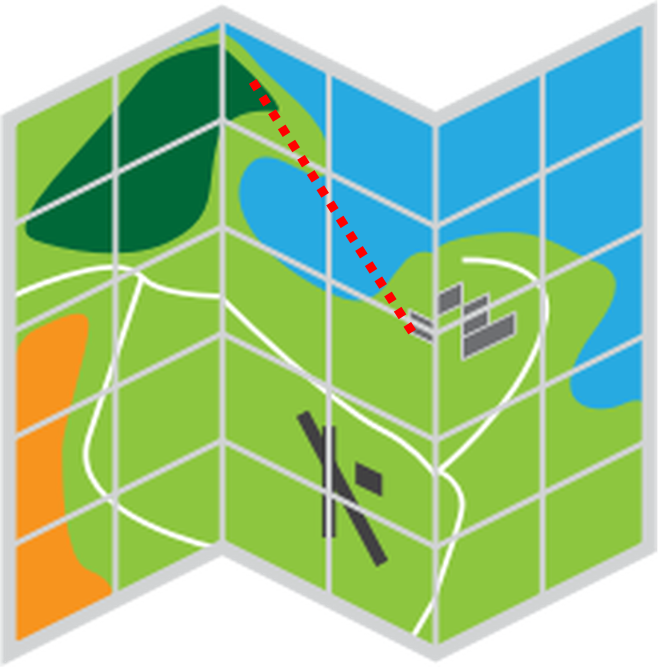
\includegraphics[width=0.7\textwidth]{img/map_icon_markers}  
	\end{center}
	\notesonly{\captionof{figure}{Distances from the viewpoint of the standard gradient.}}
\end{minipage}
\hfill
\begin{minipage}{0.45\textwidth}
	\begin{center}
		\includegraphics<2>[width=0.9\textwidth]{img/globe-icon-2-publicdomain_markers}  
	\end{center}
	\notesonly{\captionof{figure}{Taking the ``arc'' of the surface into account.}}
\end{minipage}

\end{frame}

\subsubsection{Standard gradient vs. natural gradient}

\begin{frame}{\subsubsecname}

\only<1>{
Online learning with standard gradients
\notesonly{requires us to construct a learning rate schedule to ensure we stop overshooting the solution. A decaying learning rate strategy is easier to control if the magnitudes of the gradients are more ``behaved'' so you don't suddenly get strong magnitudes that could lead to overshooting the solution.\\ 
}
\slidesonly{
\begin{itemize}
\item can overshoot the solution if we keep a constant learning rate
\item use a decaying learning rate schedule to prevent overshooting
\item a decaying learning rate strategy still sensitive to the magnitude of the gradient,
\end{itemize}
still prone to overshooting.
}
}
\only<2->{
The natural gradient enables \emph{comparable learning steps over time}\footnote{For a more detailed explanation and justification for the natural gradient, see \citep{amari1998natural}}.
It allows for a more stable, therefore efficient, and faster learning rule (no matrix inversion for $\vec W$ in Infomax'
  necessary) to do steepest ascent under normalized step size.%\notesonly{ (cf. lecture slides 2.2.1 for details)}
  
\slidesonly{
\only<2>{
\begin{equation}
	\frac{\partial e^{(\alpha)}}{\partial \mathrm{w}_{ij}}
	= \underbrace{ \big( \vec{W}^{-1} \big)_{ji} }_{
		\substack{ \text{costly} \\ \text{computation}} }
		+ \underbrace{  
			\frac{ \widehat{f}_i^{''} \bigg( \sum\limits_{k = 1}^N 
				\mathrm{w}_{ik} \mathrm{x}_k^{(\alpha)} \bigg)
			}{\widehat{f}_i^{'} \bigg( \sum\limits_{k = 1}^N 
			\mathrm{w}_{ik} \mathrm{x}_k^{(\alpha)} \bigg)}
			 }_{ \coloneqq \varphi_i^{(\alpha)} }
		\cdot \mathrm{x}_j^{(\alpha)}
		%\label{eq:gradstandardonline}
\end{equation}
}
}
  
\begin{equation}
	\Delta \vec{W} = \varepsilon \frac{ \overbrace{\partial e}^{
		\substack{	\text{``original''} \\ 
				\text{gradient}} }}{\partial \vec{W}}
		\underbrace{ \vec{W}^\top \vec{W} }_{
			\substack{	\text{normalization} \\
					\text{of step size}} }
					\label{eq:addnatgradient}
\end{equation}
}

\only<3>{
\notesonly{Applying \eqref{eq:addnatgradient} to the standard gradient in \eqref{eq:gradstandardonline}, }the natural gradient for Infomax becomes:

\begin{equation}
	\Delta \mathrm{w}_{ij} = \varepsilon \sum\limits_{l = 1}^N
	\left\{ \delta_{il} 
	+ \frac{ \widehat{f}_i^{''} \Big( \sum\limits_{k = 1}^N 
			\mathrm{w}_{ik} \mathrm{x}_k^{(\alpha)} \Big)
			}{\widehat{f}_i^{'} \Big( \sum\limits_{k = 1}^N 
			\mathrm{w}_{ik} \mathrm{x}_k^{(\alpha)} \Big)}
	\sum\limits_{k = 1}^N \mathrm{w}_{lk} \mathrm{x}_k^{(\alpha)}
	\right\} \mathrm{w}_{lj}
\end{equation}
}


\slidesonly{
\begin{center}
	\includegraphics<1>[width=0.5\textwidth]{img/section2_fig17}  
\end{center}
}



\end{frame}


% -----------------------------------------------------------------------------
\newpage

\subsection{Choice of transfer function}

\begin{frame}{\subsecname}
%\subsection{Choice of $\widehat{f}_i$:}
The true distribution is typically unknown, 
but likely to have a probability density with one maximum (i.e. peaky function)
$\leadsto$ cdf of this unknown source distribution will be roughly sigmoidal.\\

A typical choice to resemble the cdf of such a peaky function:

\slidesonly{
\begin{center}
	\includegraphics<1>[width=0.7\textwidth]{img/section2_fig15}  
\end{center}
}
\only<2>{

\svspace{-10mm}

\begin{equation} \tag{logistic function}
	\widehat{f}_{(y)} = \frac{1}{1 + \exp(-y)}
\end{equation}
\begin{equation}
	\frac{\widehat{f}_{(y)}^{''}}{\widehat{f}_{(y)}^{'}}
	= 1 - 2 \widehat{f}_{(y)}
\end{equation}
Observation: ICA is fairly robust against false choice of $\widehat{f}$.

\begin{itemize}
	\itR however: if $\widehat{f}_i$ deviates too strongly from its true
		shape, the fixed point may become unstable
	\itR if in doubt (and enough training data is available)
	\begin{itemize}
		\itl make a parametrized ansatz for $\widehat{f}_i$
		\itl estimate parameters in addition to $\vec{W}$
	\end{itemize}
\end{itemize}
}

\end{frame}

\mode*

%\clearpage

\section{References}
\begin{frame}[allowframebreaks] \frametitle{References}
	\scriptsize
	\bibliographystyle{plainnat}
	\bibliography{bibliography}
\end{frame}

\end{rightcolumn}
\end{paracol}

\end{document}
